% Chapter Template

\chapter{Efficacy Transition Pathways} % Main chapter title

\label{etp} % For referencing this chapter elsewhere, use \ref{etp}

%----------------------------------------------------------------------------------------
%	SECTION 1
%----------------------------------------------------------------------------------------

\section{Introduction}
\label{etp:Introduction}

Phase \RN{2} trials build upon the work of early Phase \RN{1} trials where preliminary information is obtained regarding the safety profile and dose schedule of a treatment. The key output from a Phase \RN{1} trial is the MTD (Maximum Tolerated Dose), TD\%\% (target dose at some pre-specified level), RP2D (Recommended Phase \RN{2} Dose) or OBD (optimal biological dose) i.e. some dose-level that can be taken forward for future testing. In Phase \RN{2} trials the focus shifts away from toxicity and looks more towards efficacy of these new treatments at the dose-levels previously defined \cite{berryBayesianAdaptiveMethods2010}. The purpose of phase \RN{2} trials is to usually see if a new treatment or intervention works and establish if there is a efficacy signal. More specifically they aim to determine if there is a sufficient level of efficacy to warrant further research in for example a Phase \RN{3} setting \cite{juliousIntroductionStatisticsEarly2010}. In addition to assessing efficacy there is also opportunity to further explore the toxicity profile of the treatment as in comparison to Phase \RN{1} trials Phase \RN{2} trials are typically conducted using a larger sample size.  

Phase \RN{2} trials can be categorised further, dependent on the primary aims of the trial. Single-arm trials can be classified as Phase \RN{2} A trials, here a sample of patients would be given the experimental treatment and efficacy would be assessed. There are also multi-arm trials which may randomise patients to multiple experimental treatments or between an experimental treatment and standard of care. Efficacy would then be compared across the different arms. These types of trials are commonly referred to as Phase \RN{2} B trials. 

Generally speaking Phase \RN{2} trials should be efficient and quick such that we can progress to Phase \RN{3} as quickly as possible or drop any ineffective treatments. The output from a Phase \RN{2} trial should be either a 'GO' or 'No GO' decision i.e should we or should we not proceed to later phase testing based on the data observed in this trial. One of the more important aspects of these trials is that we don't want to make any incorrect decisions and if there is an effective treatment that is being investigated we want to make sure that it is taken forward into Phase \RN{3}.

An example of a Phase II single arm trial design is depicted in Figure \ref{fig_etp:phase2_singlearm_example}. For single-arm Phase \RN{2} trials eligible patients come into the trial and all of them will be allocated to the new treatment. Once they have completed their treatment period we would then assess the effectiveness of that treatment using some measure of success. Looking at the outcome of success in each patient the success rate or proportion of success can then be determined. In the single arm setting, this success rate is then compared to some sort of benchmark, which is determined from either historical data or clinical input.


\begin{figure}[h!]
	\centering
	\caption{Example of a Phase 2 single arm trial design.}
	\label{fig_etp:phase2_singlearm_example}
	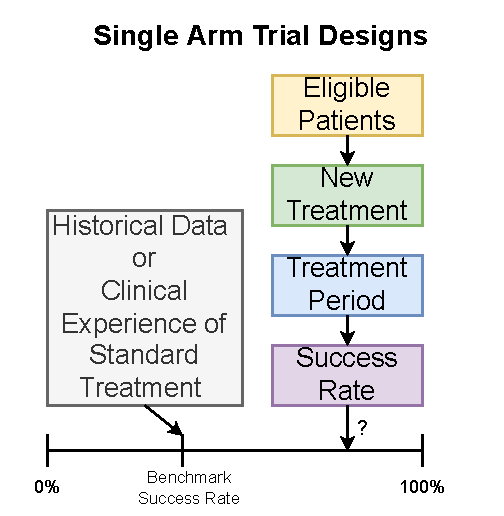
\includegraphics[width=0.75\textwidth]{ETP-Phase2SingleArmExample}
\end{figure}

The primary outcome measure for a trial like this should be some short-term binary outcome either success or failure. The outcome measure selected should be chosen such that you expect the treatment to have an effect on that. Typically these are surrogates for longer-term efficacy measures. So, if we see a success in the Phase II trial we would hope there would also be some long-term benefits for patients as well. In the oncology setting Phase III trials typically will look at outcomes such as survival times but in the previous Phase II trials response or change in tumour size may have been used as outcomes.

There are many classical frequentist approaches which can be applied to Phase \RN{2} trials such as the Flemming A'Hern, Simons two-stage or Bryant and Day designs. However, there exist complex and innovative designs that are adaptive in nature and allow for more frequent interim analyses so decisions can be made faster. 

One approach is Bayesian and utilises a Beta-Binomial conjugate analysis to estimate a  response rate for a binary outcome. Posterior probabilities can be used to inform decision making and predictive probabilities can be used during interim analyses in a similar manner. This is typically done using pre-specified decision rules.

Whilst mathematically simple to implement a design such as this has similar drawbacks to dose-finding methodologies that have been previously discussed. Due to its flexibility there may be some issues with parametrising the design, in this case would mean selecting the correct decision rules. A Bayesian approach may be less familiar than traditional frequentist approaches that are more commonly used. It may also be hard to understand why certain decisions are being made during interim and final analyses.  

One potential solution to these problems was devised by Lucinda Billingham who developed Efficacy Transition Pathways (ETPs) a novel visualisation tool to aid the design and interpretation of these types of trial designs. ETPs extend on the idea of dose transition pathways, which solves for many of the same issues in dose-finding trials. 

In this chapter we will explore the components that go into constructing an ETP for a Beta-Binomial conjugate analysis. We will detail how ETPs can be used in a trial setting with an illustrative example. Finally, we also provide details on a web application that can be used to produce ETPs and acts as an educational tool to explain what they are. 

%----------------------------------------------------------------------------------------
%	SECTION 2
%----------------------------------------------------------------------------------------

\section{Beta-Binomial Conjugate Analyses}
\label{etp:BBConjugateAnalysis}

Bayesian methods are an alternative way of thinking about evidence, data and statistics compared to the traditional frequentist approach. The Bayesian approach could be considered more intuitive and has some advantages that make it useful for analysing clinical trials. 

The fundamentals of Bayesian statistics are well defined in the literature as well as its application to clinical trials and health research. Bland and Altman \cite{blandBayesiansFrequentists1998} discuss the differences between a Bayesian or a frequentist approach. Spiegelhalter et al. \cite{spiegelhalterIntroductionBayesianMethods1999} detail the underlying philosophy behind Bayesian methods along with its application in health technology assessment. General Bayesian methods are described in more detail in books by Lee \cite{leeBayesianStatisticsIntroduction2012} and Bernado and Smith \cite{bernardoBayesianTheory2009}. It should be noted, these are just a few examples from the literature.    

The Bayesian paradigm doesn’t regard parameters, things we don’t know like a treatment effect ($\theta$), as fixed. These are instead thought of to be uncertain. Bayesian statistics uses probability to express this uncertainty. Since $\theta$ is unknown, it has a probability distribution. 

Bayesian analysis takes into account prior information on $\theta$ which also has the form of a probability distribution. This is combined with the likelihood of the data, Y given $\theta$, to produce a posterior probability distribution of $\theta$ given Y. So, data is collected to find out about the parameter. This data can be regarded as known and fixed and is used to estimate the unknown parameter. In Bayesian statistics, we estimate the probability of the parameter given the data.

Once a posterior distribution is established inferences can then be made about $\theta$. However, this may require numerical integration of the posterior distribution which may be difficult or impossible to evaluate analytically. An option around this is to use conjugate priors. If the posterior distribution and the prior distribution are from the same probability distribution family these can be referred to as conjugate distributions and the prior as a conjugate prior. Conjugate priors are algebraically easier to deal with and allow for easier interpretation of the posterior distribution. 

One example of this is what is commonly referred to as the Beta-Binomial conjugate. This is where the prior and posterior distributions take the form of a Beta distribution and the likelihood or data is Binomial. 

Binomial data has two possible outcomes. For example, a coin toss has two outcomes either its head or its tails. In the context of a Phase II single arm trial, this could be either a success/failure to some new treatment or response/no response. When this is combined with a Beta prior distribution we get a posterior Beta distribution. From this, we can then make probability statements about the treatment effect.

Following the explanation by Lee \cite{leeBayesianStatisticsIntroduction2012} of a Beta conjugate prior for a binomial distribution. Consider a parameter of interest $\theta$ that represents some treatment effect. More specifically, for binomial data in a single arm Phase \RN{2} clinical trial, lets say the parameter $\theta$ is the probability of response in a number of patients following a some new treatment. Each patient can experience either a response or no response, with the same probability of response and each patient being independent from each other. For a fixed sample size with $n$ patients and number of responses ($y$) we have: 

\begin{equation}
	Y \sim \text{Binomial}(n, \theta)
\end{equation}

So, $y$ is from a binomial distribution which produces the following likelihood: 

\begin{equation}
	L(\theta) = P(y|\theta) = {n \choose y}\theta^y (1-\theta)^{n-y} \; \; \; \; (y = 0,1,\ldots,n)
\end{equation}

If the prior for $\theta$ is from a Beta distribution such that 

\begin{equation}
	\label{eq_etp:betaprior}
	P(\theta) = \text{Beta}(a,b)
\end{equation}

then the posterior distribution is also from a Beta distribution and can be expressed as 

\begin{equation}
\label{eq_etp:betaposterior}
	P(\theta|y) = \text{Beta}(a+y,b+n-y)
\end{equation}

To avoid confusion with the prior we will let $\alpha = a+y$ and $\beta = b+n-y$ which gives

\begin{equation}
	\label{eq_etp:betaposterior2}
	P(\theta|y) = \text{Beta}(\alpha,\beta)
\end{equation}

Bayesian inference can then be used for estimation and decision making. Features such as the mean and  variance of the treatment effect $\theta$ can be  estimated from the posterior distribution given in equation \ref{eq_etp:betaposterior2}. For the posterior distribution of $\theta \sim Beta(\alpha,\beta)$ the mean, variance and mode are.

\begin{equation}
\label{eq_etp:betamean}
	E[\theta] = \frac{\alpha}{\alpha + \beta} 
\end{equation}

\begin{equation}
\label{eq_etp:betavar}
	Var[\theta] = \frac{\alpha\beta}{(\alpha+\beta)^2 (\alpha+\beta+1)}
\end{equation}

\begin{equation}
	\label{eq_etp:betamode}
	mode[\theta] = \frac{\alpha - 1 }{\alpha + \beta - 2} 
\end{equation}
 
The proofs for these formula are relatively simple and can be found in \cite{sochBookStatisticalProofs2020}. There exists no closed formula for the median however this can still be calculated using the density function of a Beta distribution. If we take $\theta^m$ to be the median then, the median is the value that solves 

\begin{equation}
	P(\theta < Median) = 0.5 = \int_{0}^{\theta^m} \theta^{\alpha-1}(1-\theta)^{\beta-1}d\theta
\end{equation}

Alternatively, there is a closed form approximation to the median presented by Kerman \cite{kermanClosedformApproximationMedian2011} which is as follows 

\begin{equation}
	median[\theta] \approx \frac{\alpha - \frac{1}{3}}{\alpha + \beta - \frac{2}{3}}
\end{equation}

We can also establish credible intervals or make other probability statements in a similar manner. 
Then pre-specified rules based on these direct probabilities from the posterior can be used for decision making purposes. For example, if 

\begin{equation}
	\label{eq_etp:betafinaldecrule}
	P(\theta > c |y) \geq q  \; \; \; \; \text{then GO else No GO}
\end{equation}


where $c$ is some target level of treatment effect and $q$ is some threshold of sufficient evidence. This probability can be calculated from the density function of the Beta distribution from $c$ to $\infty$. 

\begin{equation}
	P(\theta > c | y) = \int_{c}^{\infty}\theta^{\alpha-1}(1-\theta)^{\beta-1}d\theta
\end{equation}

It should be noted that $\int_{0}^{1}\theta^{\alpha-1}(1-\theta)^{\beta-1}d\theta = 1$, so $\theta$ has an upper bound of 1. Appropriate decision criteria, i.e. values for $c$ and $q$, can be determined and evaluated via simulations.

%-----------------------------------
%	SUBSECTION 1
%-----------------------------------

\subsection{Illustrative example to showcase a Beta-Binomial design} 
\label{etp:BBIllEx}
In this section we will detail an example to show how a Beta-Binomial conjugate analysis would work in practice and how its used to make decisions. 

Consider a trial in which we are trying to evaluate the efficacy of some new treatment. This will be done using an outcome measure of response. Patients can either be considered a responder or a non-responder. The treatment effect will be the response rate and will be analysed using a Beta-Binomial conjugate model. 

To conduct the analysis and make a GO or No GO decision a prior and decision criteria needs to be specified. For simplicity a minimally informative Beta(1,1) prior will be used. This represents a 50\% response rate from a group of two patients. The following decision rule will also be used $P(\theta  \geq 30\%) \geq 0.9$, where $\theta$ is the treatment effect (response rate). So, if there is a greater than  90\% chance that the true response rate is at least 30\% this will be considered sufficient evidence to warrant a GO decision. 

Now assume that 30 patients were recruited 16 of which had a response. Using equation \ref{eq_etp:betaposterior} we can establish that the posterior distribution for the treatment effect is $P(\theta) = \text{Beta}(17, 15)$. From this we can then calculate summary estimates, which are presented in Table \ref{tab_etp:bb_sum_est}.

\begin{table}[H]
	\centering
	\caption{Summary estimates of response rate with 30 patients and 16 responses. }
	\label{tab_etp:bb_sum_est}
	\begin{tabular}{cc}
		\hline
		\textbf{Summary Estimate}                   &              \\ \hline
		\multicolumn{1}{c|}{Mean}                   & 0.531        \\
		\multicolumn{1}{c|}{Median}                 & 0.532       \\
		\multicolumn{1}{c|}{Mode}                   & 0.533          \\
		\multicolumn{1}{c|}{Variance}               & 0.008        \\
		\multicolumn{1}{c|}{95\% Credible Interval} & 0.360, 0.698 \\ \hline
	\end{tabular}
\end{table}

From these estimates we can say, based on the data that is observed (16 responses in 30 patients), the response rate is 53\% with a 95\% credible interval (36\%, 70\%). The probability of the response rate being at least 40\% can also be calculated. In this example it is 99.7\%. As this value is greater than the threshold of 90\%  we can say there is sufficient evidence to warrant a GO decision.

This can also be illustrated as shown in Figure \ref{fig_etp:bb_dec_rule1}. The blue shaded region highlights the upper 90\% of the distribution. In this scenario with this decision criteria, as the entire region does not cross the target response rate of 30\% we have a GO decision. We can see that there is a greater than 90\% chance that the response rate is greater than 30\%. 

 \begin{figure}[h!]
 	\centering
 	\caption{Posterior distribution of response rate with decision criteria.}
 	\label{fig_etp:bb_dec_rule1}
 	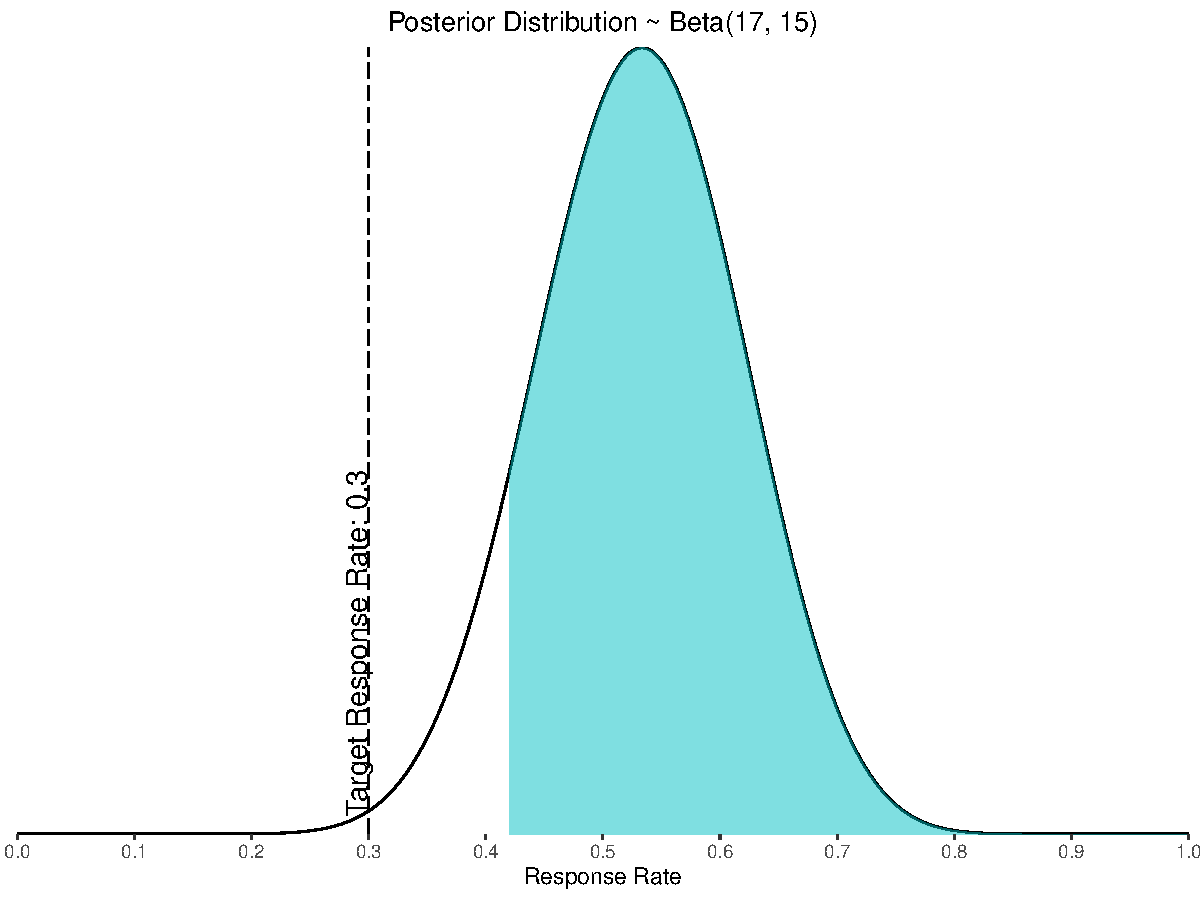
\includegraphics[width=\textwidth]{ETP-BetaBinomialDecRule1}
 \end{figure}

In practice decision rules should be decided before the trial starts. This is typically done via the evaluation of simulations. Multiple scenarios corresponding to different true response rates can be investigated. The probability of making a correct decision can then be calculated. This represents the power of our design. For scenarios with low true response rates (relative to the target response rate) we want the probability of making a No GO decision to be high. Similarly, for scenarios with high true response rates we want the probability of making a GO decision to be high. The decision rule parameters, the target response rate and probability threshold can then be adjusted to ensure the design is making appropriate decisions in these scenarios. 

Simulations can also be used to evaluate the choice of prior as well. A variety of different priors can be used dependent on the trial. A prior like the Beta(1,1) is typically described as minimally informative. This means that if the data observed is reasonably large the likelihood will dominate and have more influence on the posterior. So, if we observe a really strong treatment effect this will be reflected in the posterior. 

A sceptical prior can be used when we are sceptical about the treatment producing large treatment effects. These are typically centred around a low treatment effect whilst still leaving some scope for their to be plausible positive treatment effect. The opposite of this would be a enthusiastic prior. Here the prior would be centered around a high treatment effect whilst allowing some possibility for a negative treatment effect.

Priors can also be evidence based or elicited. Evidence based priors will use results or data from previous trials to inform the choice of prior. These can then be adjusted to account for any potential biases. Elicited priors are decided based on discussions with a group of experts. 

Figure \ref{fig_etp:bb_example_priors} shows the effect that different priors can have on the estimation of the treatment effect. Our example with 16 responses and a minimally informative prior is shown in the first plot. Here we can see the median response rate is 53.2\% and the probability of the response rate being greater than 30\% is greater than 90\% meaning we have a go decision. The minimally informative prior is indicated by the red line and is essentially a uniform distribution. Assuming we still have 16 responses, we can see that when a sceptical Beta(2,8) prior is implemented the posterior distribution changes from Beta(17,15) to Beta(18,22). This shifts the posterior such that the new estimated median response rate is 44.9\%. However even with a sceptical prior we can still see we meet the criteria for a GO decision with a probability of 0.976 that the response rate is greater than 30\%. Then with an enthusiastic prior the posterior shifts in the other direction. So, with the same 16 responses but an enthusiastic prior the estimate of the response rate is 57.6\%. Again, the decision criteria is also met in this instance as well.    

 \begin{figure}[h!]
	\centering
	\caption{Posterior distribution of example under different priors.}
	\label{fig_etp:bb_example_priors}
	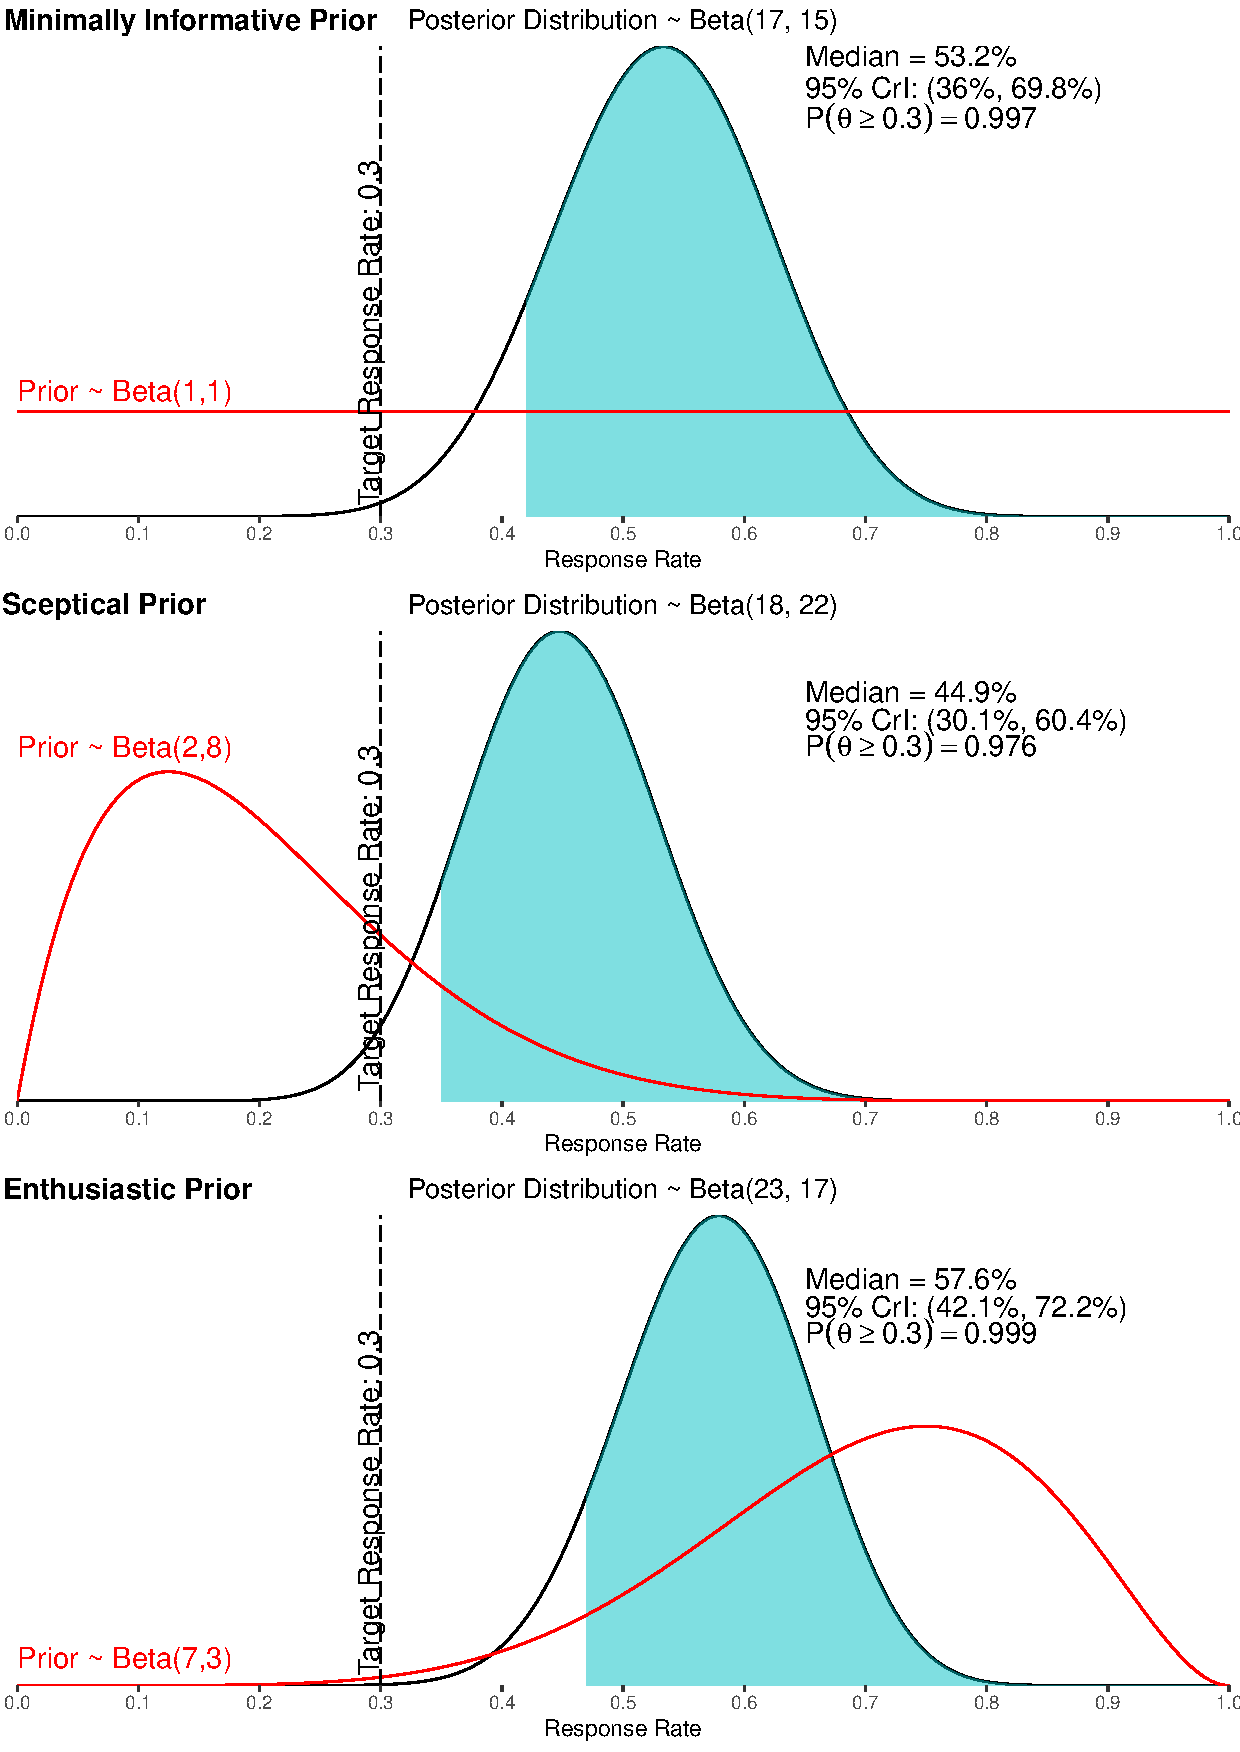
\includegraphics[width=\textwidth]{ETP-BetaBinomialPriors}
\end{figure}

In this example the choice of prior did not impact the decision that would be made. However, if the decision rule was different or the number of responses seen was less this could change. As part of some trials a sensitivity may be conducted to check the results and decisions of a trial with a different prior. As stated before simulation work is used to establish the most appropriate decision criteria and priors can be sourced from available evidence or elicited. The simulations should be conducted with the priors in mind as well as any sensitivity analyses that may be planned.   

Once the decision rule and prior have been specified the minimum number of responses required to make a GO decision could also be calculated. In our example here this number is 13. So, we would need to observe a minimum of 13 responses to make a GO decision out of 30 patients. To make these trial designs more efficient interim analyses can be included. This will allow the trial to look at the data at an earlier time point and potentially make a decision earlier as to whether the trial should continue. In the next section we look at how the predictive probability of success (PPOS) is used to make decisions at interim analyses. 

%-----------------------------------
%	SUBSECTION 3
%-----------------------------------

\subsection{Interim analyses and Predictive Probability of Success}

There are several different methods in which interim analyses can be incorporated into a single-arm Phase \RN{2} clinical trial. One method that can be used in the context of a Beta-Binomial conjugate analysis utilises PPoS. This works by evaluating the data at pre-specified time points or after a certain intervals of patients have been recruited. At these time points we can determine whether or not we have observed enough responses to warrant continuing with the trial based on the overall minimum responses we would need for a final GO decision. More explicitly the PPoS is the probability of the trial being considered a success given the current data observed at the interim analysis. This is calculated by predicting the future number of responses in the patients yet to be recruited based on the data that has already been observed. 

In section \ref{etp:BBConjugateAnalysis} we detailed how a Beta-Binomial conjugate analysis works in practice. Here, we will extend that to show how PPoS and an interim analysis can be incorporated into this trial design following the explanation of Berry et al. \cite{berryBayesianAdaptiveMethods2010}. 

Consider for a fixed sample of size $n$ patients an interim analysis that will be conducted after $n_{int}$ patients, such that $n_{int} < n$. Again, the parameter of interest, treatment effect or response rate will be represented by $\theta$. Let the number of responses $x$ among the $n_{int}$ patients follow a binomial distribution: 

\begin{equation}
	X \sim \text{Binomial}(n_{int},\theta) 
\end{equation}

Let $Z$ be the number of responses in the remaining $m$ patients, where $m = n - n_{int}$. When $Z = i$, where $i = 1, ..., m$, the posterior distribution can be expressed as 

\begin{equation}
	P(\theta|x,Z=i) = \text{Beta}(a+x+z, b+n-x-z)
\end{equation}

Where $a$ and $b$ are parameters from the Beta prior distribution, see equation \ref{eq_etp:betaprior}. 

Suppose we have a decision rule where a GO decision is made if the posterior probability of $\theta$ exceeds some pre-specified target treatment effect/ response rate $c$ with a probability greater than some threshold $q$ (as defined in equation \ref{eq_etp:betafinaldecrule}).

The predictive probability of success (PPoS) can be calculated as follows. Let $B_i = P(\theta > c |x, Z=i)$ and $I_i = I(B_i \geq q)$ be an indicator variable taking a value of 1, if the criteria $B_i \geq q$ is satisfied or 0 otherwise. Then we have 

\begin{equation}
	\begin{aligned}
		\text{PPoS} & = E\{I[P(\theta > c |x,Z) \geq q]|x \} \\
		& = \int I[P(\theta > c |x,Z) \geq q]dP(Z|x) \\
		& = \sum_{i =0}^{m} P(Z = i|x)I[P(\theta > c |x,Z=i) \geq q] \\
		& = \sum_{i =0}^{m} P(Z=i|x)I(B_i \geq q) \\
		& = \sum_{i =0}^{m} P(Z=i|x)I_i
	\end{aligned}
\end{equation}

Where $P(Z = i | x)$ is the probability of observing $Z$ responses in $m$ patients based on a beta probability distribution with parameters $a+x$ and $b+n_{int}-x$. This can be calculated from the probability mass function

\begin{equation}
	\begin{aligned}
		f(Z = i|m, a+x, b+n_{int}-x) & = {m\choose z} \frac{\text{Beta}(a+x+z, b+n_{int}+m-x-i)}{\text{Beta}(a+x, b+n_{int}-x)} \\
		& = {m\choose z} \frac{\text{Beta}(a+x+z, b+n-x-i)}{\text{Beta}(a+x, b+n_{int}-x)} \\
	\end{aligned}
\end{equation}

The Beta functions can be further simplified or alternatively expressed using the gamma function. Note $\Gamma(k) = (k-1)!$

\small
\begin{equation}
	\begin{aligned}
		f(Z = i) & = \frac{m!}{z!(m-z)!}\cfrac{\cfrac{\Gamma(a+x+z)\Gamma(b+n-x-z)}{\Gamma(a+b+n)}}{\cfrac{\Gamma(a+x)\Gamma(b+n_{int}-x)}{\Gamma(a+b+n)}} \\
		& = \frac{\Gamma(m+1)}{\Gamma(z+1)\Gamma(m-z+1)}\frac{\Gamma(a+x+z)\Gamma(b+n-x-z)}{\Gamma(a+b+n)}\frac{a+b+n_{int}}{\Gamma(a+x)\Gamma(b+n_{int}-x)}
	\end{aligned}
\end{equation}
\normalsize

The process to calculate the PPoS starts with the quantity $B_i$ which represents the probability that the response rate is greater than some target $c$ given $x$ responses in $n_{int}$ patients and assuming $i$ future responses in the remaining $m$ patients. The quantity $B_i$ is then compared to our probability threshold $q$ which provides a value for the indicator variable $I_i$ and informs us if the trial would result in a GO decision at the end of the trial dependent on the data observed and the value of $Z=i$. The indicators $I_i$ are then weighted by the probability $P(Z=i)$ and summed to give the PPoS. 

PPoS is then interpreted and used to make decisions at interim analyses. Low values of PPoS suggest there is a low probability of achieving a GO decision at the final analysis based on the data accrued so far. Similarly, a high PPoS suggests the opposite and that the trial would likely be a success based on the current data. An interim decision rule can then be implemented around values of PPoS to recommend stopping the trial early for either efficacy or futility. To stop for futility a the following rule could be imposed 

\begin{equation}
	\text{PPoS} < t  \; \; \; \; \text{then STOP for futility}
\end{equation}

Where $t$ is some PPoS acceptable probability threshold. Values of $t$ range from 0 to 1 but would typically be small. For example a value of 0.05 may be used to indicate if there is a less than 5\% chance that the response rate at the end of the trial will be greater than $c$ with some probability $q$ then the trial should stop early. 

To show how this works in practice we will extend the example shown in section \ref{etp:BBIllEx} to include an interim analysis. The same Beta(1,1) prior and decision rule $P(\theta  \geq 30\%) \geq 0.9$ will be utilised. A maximum sample size of 30 patients will be used except now an interim analysis will be performed after 15 patients have been recruited. We will use the following decision rule, such that if the PPoS $\leq 0.05$ we will recommend stopping the trial. 

Lets consider after 15 patients we observe 8 responses. We also know in the remaining $m$ patients, 15 in this scenario, there can be between 0 and 15 responses. Table \ref{tab_etp:bb_ppos_8resp} shows the calculations required to determine PPoS. 

\begin{table}[h!]
	\caption{\label{tab_etp:bb_ppos_8resp}Predictive probability of success calculations for 8 responses after 15 patients.}
	\centering
	\begin{tabular}[t]{cccc}
		\toprule
		$Z = i$ & $P(Z = i|x)$ & $B_i = P(\theta \geq 0.3 |x, Z=i)$ & $I(B_i \geq 0.9)$\\
		\midrule
		0 & 0.0006 & 0.3865 & 0\\
		1 & 0.0035 & 0.5416 & 0\\
		2 & 0.0116 & 0.6879 & 0\\
		3 & 0.0277 & 0.8076 & 0\\
		4 & 0.0524 & 0.8931 & 0\\
		5 & 0.0833 & 0.9466 & 1\\
		6 & 0.1143 & 0.9761 & 1\\
		7 & 0.1378 & 0.9905 & 1\\
		8 & 0.1470 & 0.9966 & 1\\
		9 & 0.1388 & 0.9989 & 1\\
		10 & 0.1153 & 0.9997 & 1\\
		11 & 0.0830 & 0.9999 & 1\\
		12 & 0.0503 & 1.0000 & 1\\
		13 & 0.0244 & 1.0000 & 1\\
		14 & 0.0085 & 1.0000 & 1\\
		15 & 0.0016 & 1.0000 & 1\\
		\bottomrule
	\end{tabular}
\end{table}

We can see that when the number of responses is less than five the quantity $B_i$ is less that 0.9. As such a GO decision would not be made at the final analysis. On the other hand when the number of responses is greater than or equal to five a GO decision would be achieved at the final analysis. This also aligns with what was presented before where a minimum of 13 responses would be required for a GO decision. As we had eight in the first 15 patients a minimum of five responses would be required in the subsequent 15 patients. 

The PPoS is then just the sum of the indicators of a positive trial result weighted by the probability of observing that result. This is just the sum of $P(Z = i|x)$ where $I(B_i \geq 0.9)$. Here, the PPoS is 0.9043. So, based on observing 8 responses out of 15 patients there is a 90\% chance the trial will be successful if it recruits a further 15 patients. As this PPoS value is much greater than our 5\% acceptable probability level we would not recommend stopping at the interim analysis. 

In this example we assumed that there were eight responses. However, if this was instead three the PPoS would only be 0.009. This is less than our 5\% target so would mean that the trial would recommend stopping. If the number of responses was 13 the PPoS would then be 1. This is due to our decision rule requiring a minimum of 13 responses out of 30 patients for a GO decision. As this would have been achieved in the first 15 patients the trial could be declared a success. 

The PPoS will also vary dependent on the timing of the analysis. It is also possible to incorporate multiple analyses without any additional effort. The same process to calculate PPoS can be done every five patients for example. Simulations can be used to assess and determine the best decision rule to use for PPoS and the frequency of interim analyses. 

Whilst fairly simple to calculate and implement interim analyses and decision rules for a trial design like this may be difficult for non statisticians to grasp and interpret. To aid this, for the final decision rule, we can calculate and detail explicitly how many patients or responses are required to make certain decisions. In our example, we needed a minimum of 13 responses out of 30 patients to make a GO decision. This could then be used to inform discussions with the clinicians as to whether this is appropriate or if the decision rule needs to be updated. 

For interim analyses, the same can be done but there is more data to consider. As for each interim you would need to know the minimum number of responses that would have to be observed to not stop the trial. In our example of an interim at 15 patients you would need to observe four responses to continue recruiting. Depending on how many interim analyses are specified in the trial this would have to be done multiple times.

In the next section we present a novel plot which visualises different outcomes and decisions made in a Phase \RN{2} trial using a Beta-Binomial design incorporating multiple interim analyses.   

%----------------------------------------------------------------------------------------
%	SECTION 3
%----------------------------------------------------------------------------------------

\section{Constructing Efficacy Transition Pathways}
We have explored how PPoS can be used for interim analyses to determine if the trial will be a success or not. At each interim PPoS is calculated based on the number of responses observed thus far and evaluated to see if it meets the decision criteria. Therefore there will be a minimum number of responses that have to be observed in order to continue recruitment. This is similar to how we can calculate the number of responses required at the end of the trial to warrant a GO decision. Obviously, the minimum number of responses required at each interim and the final analysis depends on the decision criteria that is specified. 

Intuitively, it is easier to understand that four responses have to be observed from 15 patients rather than a PPoS $\leq 0.05$ is needed. Through discussions with clinicians we can then calibrate our decision criteria based on these interpretations. We may want to be more strict or lenient at our interim. If the clinicians would be happy to continue recruitment after seeing only two responses we could lower the PPoS threshold, likewise if they wanted to be confident and only continue if six responses were observed we would increase the PPoS threshold. Similarly, this can also be done for the final analysis decision criteria. The acceptable probability level or target response rate could be adjusted so a specific minimum number of responses observed achieves a GO decision.  

For our example trial, in the last section, with 30 patients and only one interim this is fairly easy information to present and discuss with the clinicians. However, as more interims are added trying to understand the break points at each interim become more complex. A solution for this is ETPs. In this section we will present how they are constructed and how they can be utilised in the design and interpretation of a trial. 

In order to illustrate an ETP we will use the same example as before. However, rather than just having one interim at 15 patients we will conduct an interim every five patients. With a total sample size of 30 patients there will be five interims and one final analysis. The same decision criteria will be used as well. At each interim recruitment will stop if PPoS $< 0.05$ and at the final analysis a GO decision will be made if $P(\theta  \geq 30\%) \geq 0.9$. 

To construct an ETP we produce individual cells which contain key information about a specific outcome i.e. a certain amount of responses. If we consider our first interim at five patients, at that point there are six different possible outcomes that can be observed. Either one, two, three, four or all five of the patients had a response or none of them did. For each possible outcome we can then calculate the PPoS as well as the Bayesian estimate of the response rate and an associated credible interval. Figure \ref{fig_etp:Cell0Resp5Pat} shows what this cell would look like. 

\begin{figure}[h!]
	\centering
	\caption{ETP cell plot for 0 responses in 5 patients.}
	\label{fig_etp:Cell0Resp5Pat}
	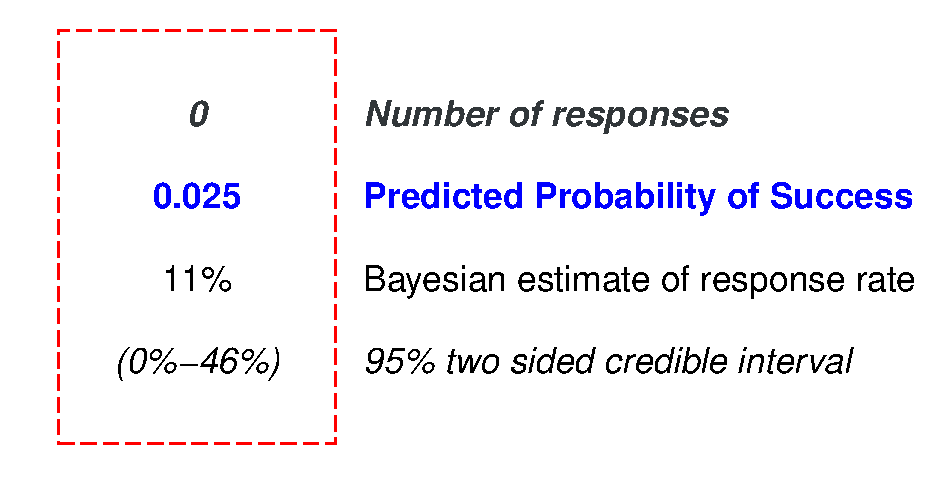
\includegraphics[width=\textwidth]{ETP-cell0Resp5Pat}
\end{figure}

The number at the top indicates the outcome for the cell, in this case the number of responses which is 0. The second row shows the PPoS in this scenario, the third row showing the Bayesian estimate of response rate and the last row shows the 95\% credible interval. For 0 responses the PPoS is 0.025 which is less than our threshold so the decision here would be to stop. This is represented by the red dashed line. From this one cell we are able to see what the decision would be at the interim analysis time point if this is the outcome that is observed. We are also able to see specifically what the PPoS and estimated response rate would be as well.  

Cells are generated for each possible outcome at each interim time point. Figure \ref{fig_etp:Cell2Resp5Pat} shows the cell for two responses in five patients. Here we can see the PPoS is 0.501 which is greater than our threshold so the decision would be made to continue recruitment. This is indicated by the green dashed line. As we put each cell together we can then clearly see the minimum number of responses required to continue recruiting.  

\begin{figure}[h!]
	\centering
	\caption{ETP cell plot for 2 responses in 5 patients.}
	\label{fig_etp:Cell2Resp5Pat}
	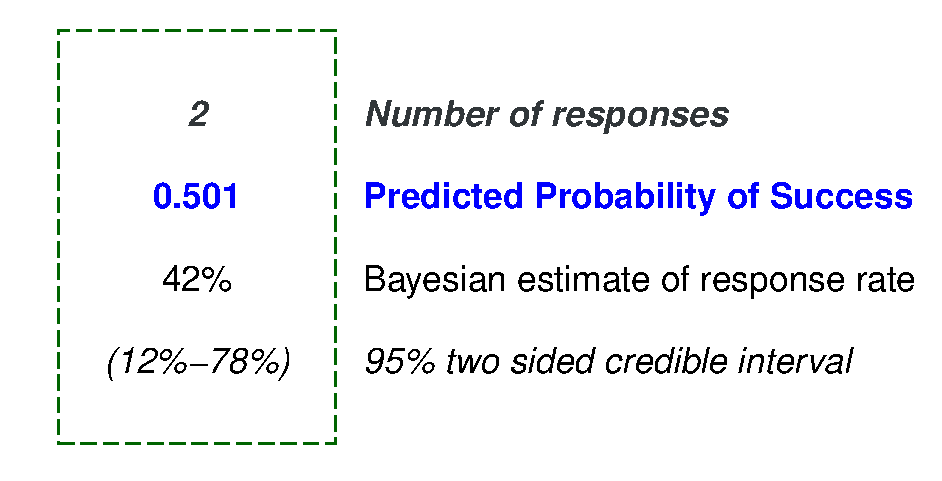
\includegraphics[width=\textwidth]{ETP-cell2Resp5Pat}
\end{figure}

This process is then repeated for each interim analysis. So, the next analysis would be at 10 patients. Here we would generate 11 cells for all the different possible outcomes (no response, one response, two responses, ..., 10 responses). The same would then be done for the analysis at 15, 20 and 25 patients. 

For the final analysis the presentation of the cells is slightly different. Here we are no longer interested in PPoS as no more patients will be recruited and rather we can just evaluate if the trial has met the decision criteria. So, in each cell rather than present PPoS the posterior probability that the response rate is greater than our target rate is presented instead. Figures \ref{fig_etp:Cell10Resp30Pat} and \ref{fig_etp:Cell14Resp30Pat} show the cells for 10 responses and 14 responses out of 30 patients respectively. In this example our $q$ is set at 0.9 so if the posterior probability is greater than that we have a GO decision. 


\begin{figure}[h!]
	\centering
	\caption{ETP cell plot for 10 responses in 30 patients.}
	\label{fig_etp:Cell10Resp30Pat}
	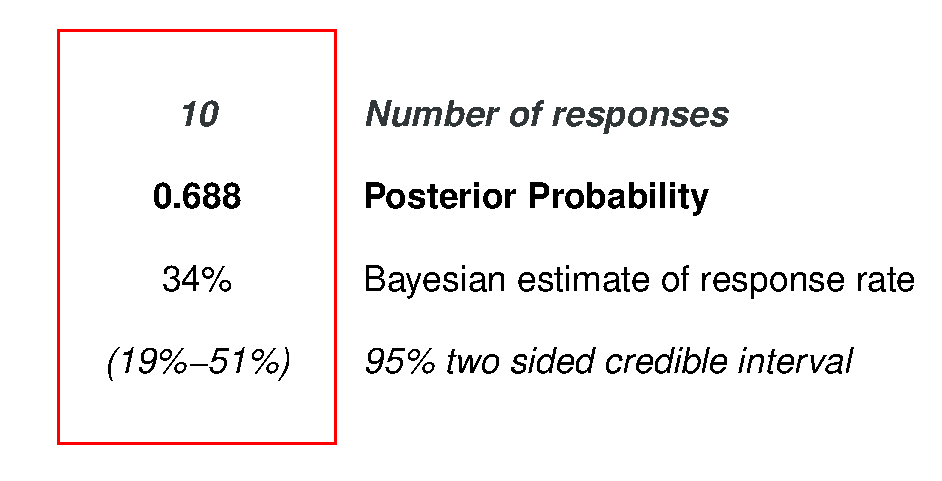
\includegraphics[width=\textwidth]{ETP-cell10Resp30Pat}
\end{figure}


\begin{figure}[h!]
	\centering
	\caption{ETP cell plot for 14 responses in 30 patients.}
	\label{fig_etp:Cell14Resp30Pat}
	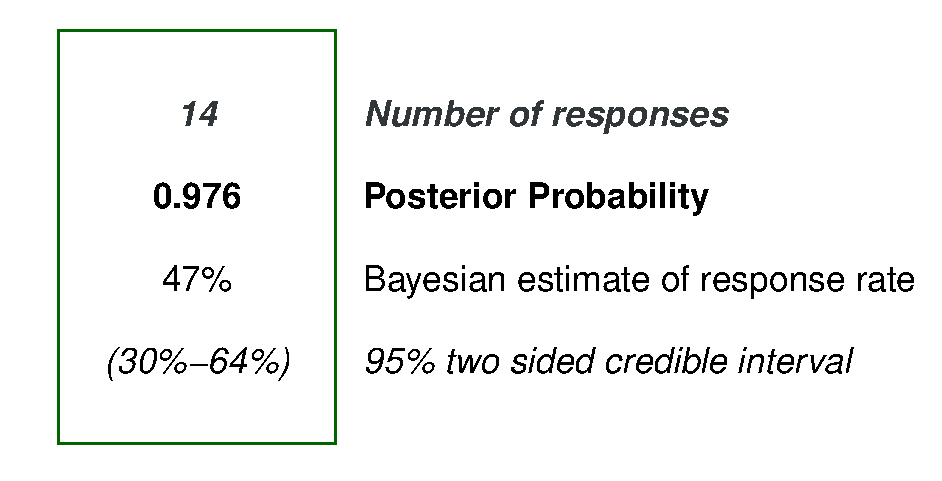
\includegraphics[width=\textwidth]{ETP-cell14Resp30Pat}
\end{figure}


The efficacy transition pathway is then constructed by grouping each cell for each interim analysis and then stacking those group of cells together. For our example trial the ETP is shown in Figure \ref{fig_etp:ConstructedETP}. Each row of cells in the ETP represents each interim analysis with the final row representing the final analysis. One adaptation made with the cells is that the confidence interval is presented across the bottom two rows in each cell just to make the figure easier to read and more scalable. 

From this figure what can clearly be seen is when we do or do not have a GO decision. At each interim of 5, 10, 15, 20, 25 patients we can see that the minimum number of responses for a GO decision is 1, 2, 4, 7 and 9 respectively. Also, for the final analysis a minimum of 13 responses is required. 

We can also evaluate some aspects of our decision rule criteria. Specifically, around $t$ our PPoS acceptable probability threshold and $q$ our threshold of sufficient evidence or the final decision. If we were to change our value of $t$ from 0.05 we can see what affect that would have on the decisions that would be made. We can identify this by looking at the PPoS in each cell for the different interims and comparing that against the new decision rule. Consider a new value of $t$ of 0.1 our interim decision rule would become PPoS $< 0.1$, so we would stop at each interim analysis if our PPoS was less than 10\%. Now the minimum number of responses for a GO decision at each interim is 1, 3, 5, 7 and 10. This has stayed the same for the interim analyses at 5 and 20 patients but has increased by 1 extra response for the other interims. We can update our ETP to reflect this change. Figure \ref{fig_etp:ConstructedETPNewPPoS} shows this new plot. The only changes here to the original ETP \ref{fig_etp:ConstructedETP} is the colour of the border around the cells for when a GO decision is made. All the calculations of PPoS, Bayesian estimates and posterior probabilities remain the same. 

Similarly, we can also check the posterior probability for the final analysis against our value of $q$. If we were to change this to 0.8 so the decision rule would now become $P(\theta  \geq 30\%) \geq 0.8$. The minimum number of responses for a GO decision at the final analysis would be 11. By looking at the final row and the cell representing the outcome for 11 patients we see here the posterior probability is 0.808. That means the probability of the response rate being greater than 30\% is 0.808 which would meet the criteria for this new decision rule. Its important to note any change made to the final analysis decision rule will have a knock on effect to decisions made at the interim analysis. This is because the final decision rule is used to calculate the PPoS. So let's say we keep the original interim analysis decision rule of stopping if PPoS $< 0.05$ but we use the new final decision rule $P(\theta  \geq 30\%) \geq 0.8$. The associated ETP for this set of rules is given in Figure 
\ref{fig_etp:ConstructedETPNewFinal}. Here the values of PPoS have changed for the interim analyses as has the minimum number of responses required for a GO decision. It is important to note that the posterior probabilities and the Bayesian estimates of response rate with it's credible interval are the same throughout these plots. They Bayesian estimates will remain unaffected by the changes in decision rules as they are calculated based on the Beta-Binomial conjugate analysis. However, the posterior probability will change if the target response rate, $c$, is different as this is just the probability that the true response rate is higher than $c$. 

Any changes made to the target response rate in the decision rule would impact the PPoS, the posterior probability and the minimum number of responses required for GO decisions at the interim and final analyses. If our target response rate was now 40\% instead of 30\% and we kept all the decision rules and parameters the same as our original example. We would have the following decision rules: stop if PPoS $< 0.05$ at each interim and GO at final if $P(\theta  \geq 40\%) \geq 0.9$. With this new target response rate at least 16 responses are required for a GO at the final analysis. The numbers at each interim also differ as well. This can be seen in Figure \ref{fig_etp:ConstructedETPNewTarget}. 

Table \ref{tab_etp:ETP_plots_summary} provides a summary of all of the ETP plots produced. This allows us to easily compare for each plot and set of decision rules the minimum number of patients required for a GO decision. This doesn't reflect all the information that is shown in each plot but just provides a brief summary. 

\begin{table}[h!]
	\centering
	\caption{Summary of the ETP figures. }
	\label{tab_etp:ETP_plots_summary}
	\resizebox{\textwidth}{!}{%
		\begin{tabular}{l|cc|cccccc}
			\hline
			\multirow{2}{*}{\textbf{Figure}} &
			\multicolumn{2}{c|}{\textbf{Decision Rules}} &
			\multicolumn{6}{l}{\textbf{Minimum Number of Responses for a GO Decision}} \\ \cline{2-9} 
			&
			\textbf{Interim} &
			\textbf{Final} &
			\textbf{N =5} &
			\textbf{N =10} &
			\textbf{N = 15} &
			\textbf{N = 20} &
			\textbf{N = 25} &
			\textbf{N = 30} \\ \hline
			\ref{fig_etp:ConstructedETP} & PPoS $< 0.05$ & $P(\theta  \geq 30\%) \geq 0.9$ & 1 & 2 & 4 & 7 & 9  & 13 \\
			\ref{fig_etp:ConstructedETPNewPPoS} & PPoS $< 0.1$  & $P(\theta  \geq 30\%) \geq 0.9$ & 1 & 3 & 5 & 7 & 10 & 13 \\
			\ref{fig_etp:ConstructedETPNewFinal} & PPoS $< 0.05$ & $P(\theta  \geq 30\%) \geq 0.8$ & 0 & 2 & 3 & 5 & 8  & 11 \\
			\ref{fig_etp:ConstructedETPNewTarget} & PPoS $< 0.05$ & $P(\theta  \geq 40\%) \geq 0.9$ & 1 & 3 & 6 & 9 & 12 & 16 \\
			\hline
		\end{tabular}%
	}
\end{table}

\begin{sidewaysfigure}
	\centering
	\caption{Example of a constructed ETP.}
	\label{fig_etp:ConstructedETP}
	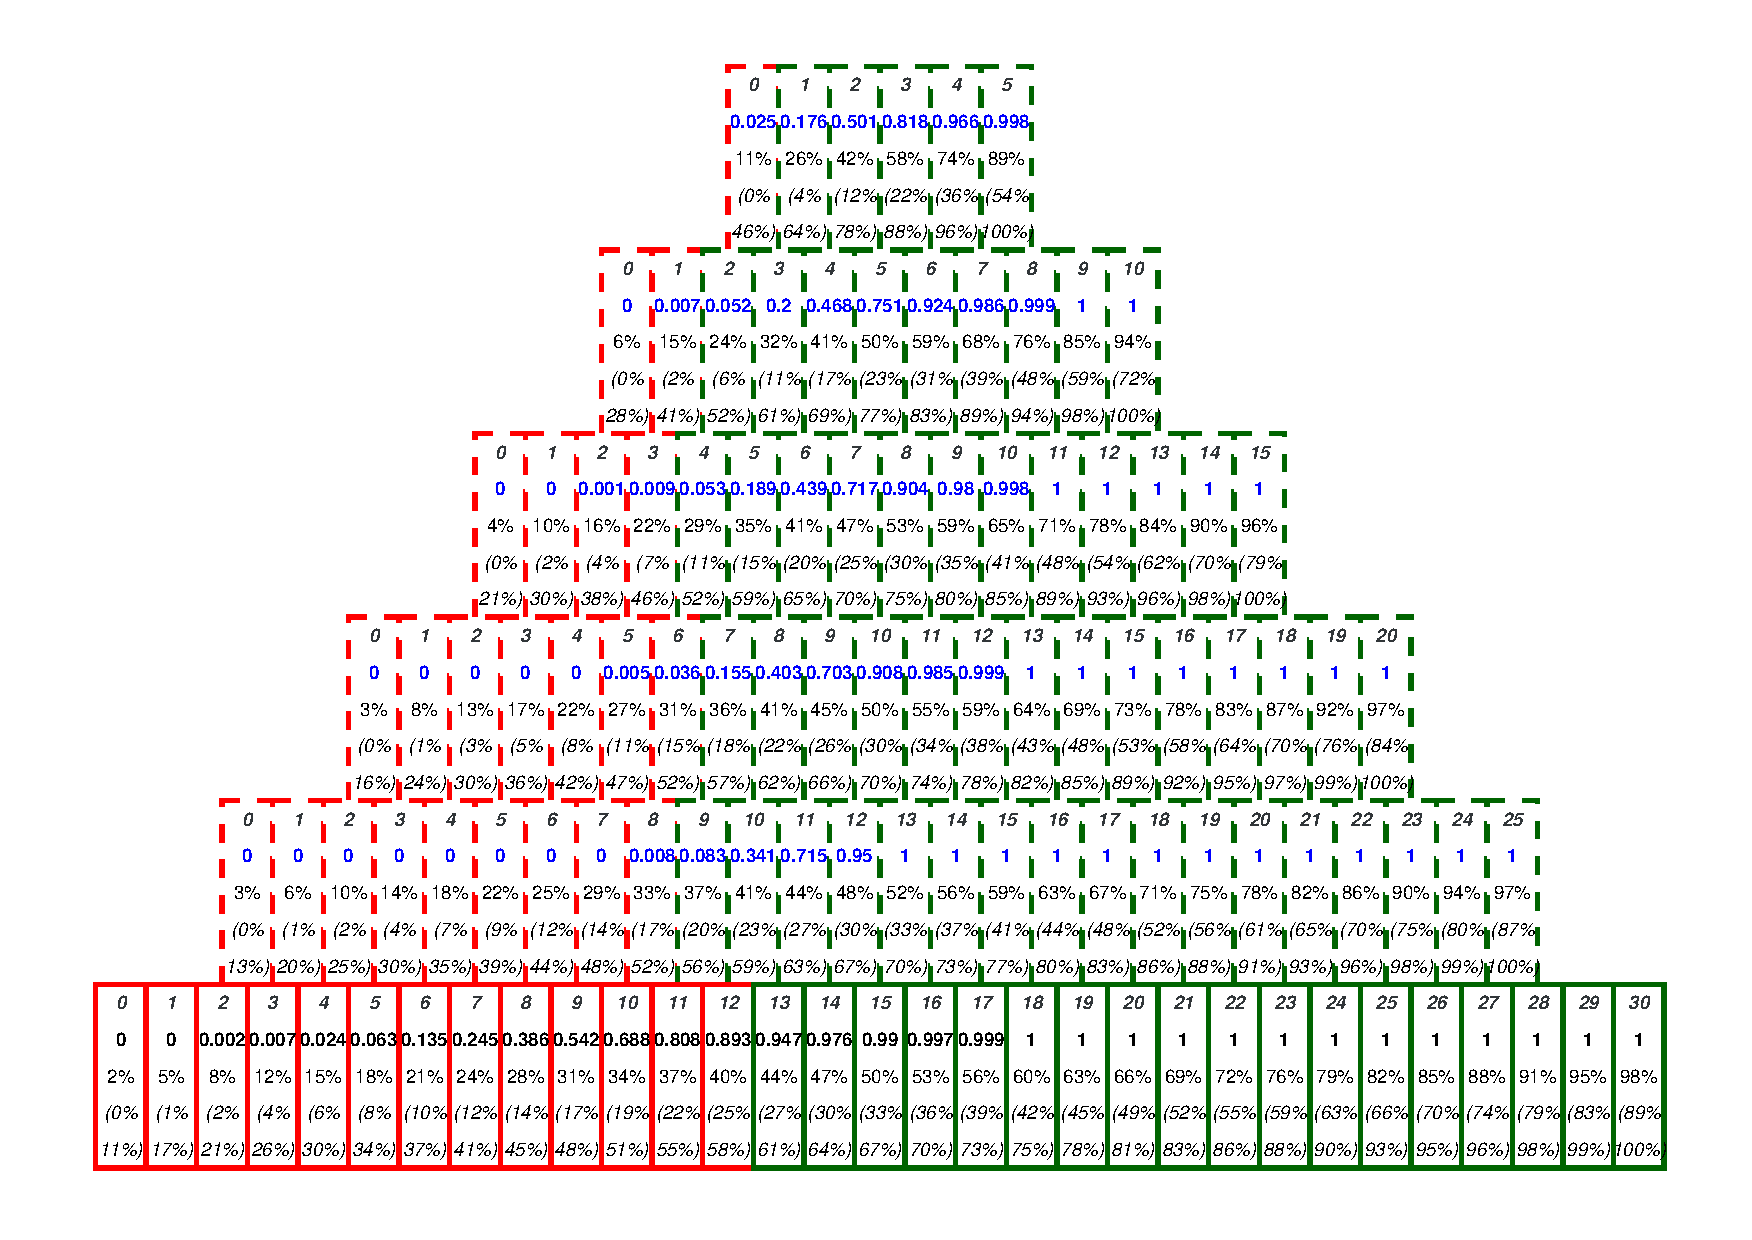
\includegraphics[width=25cm, height=15cm]{ETP-constructed}
\end{sidewaysfigure}

\begin{sidewaysfigure}
	\centering
	\caption{Example of a constructed ETP with new PPoS decision rule.}
	\label{fig_etp:ConstructedETPNewPPoS}
	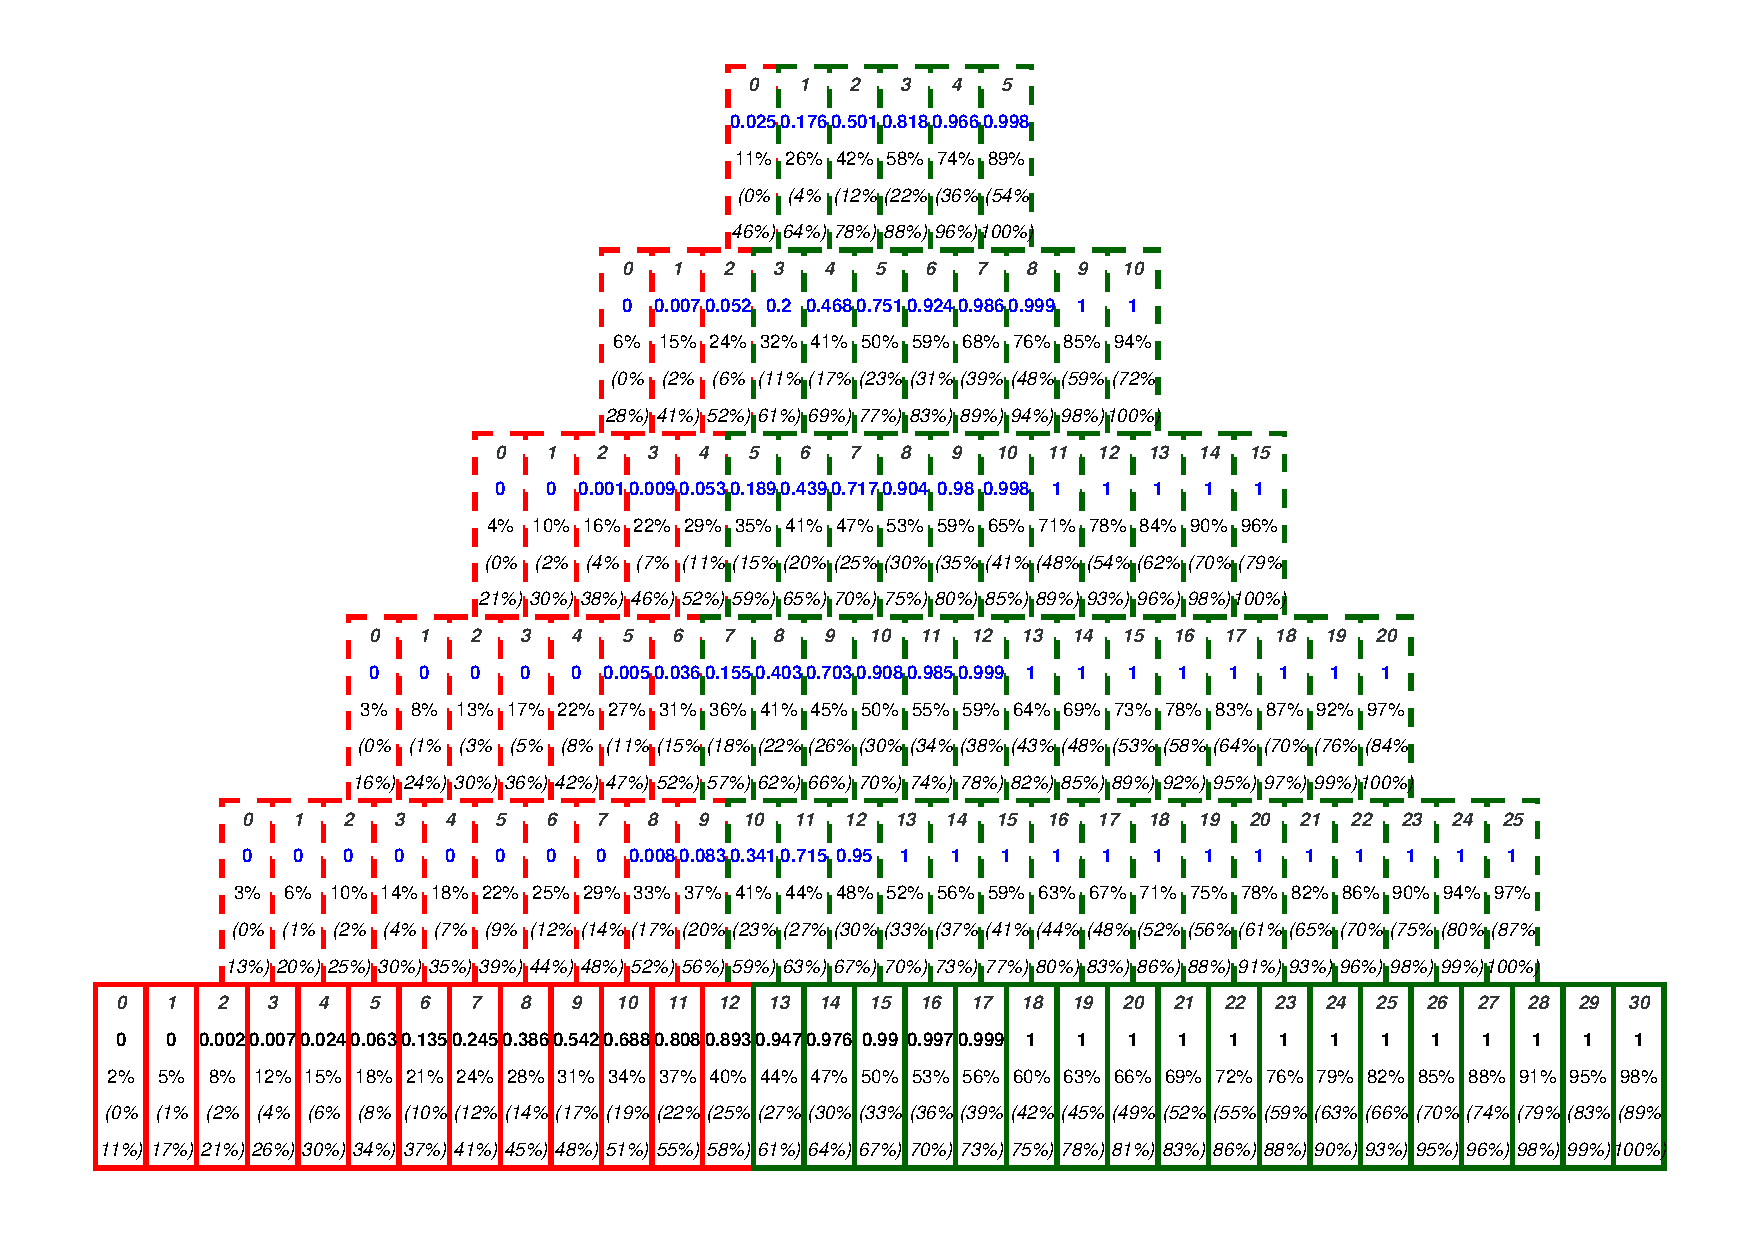
\includegraphics[width=25cm, height=15cm]{ETP-constructedNewPPoSRule}
\end{sidewaysfigure}

\begin{sidewaysfigure}
	\centering
	\caption{Example of a constructed ETP with new final decision rule.}
	\label{fig_etp:ConstructedETPNewFinal}
	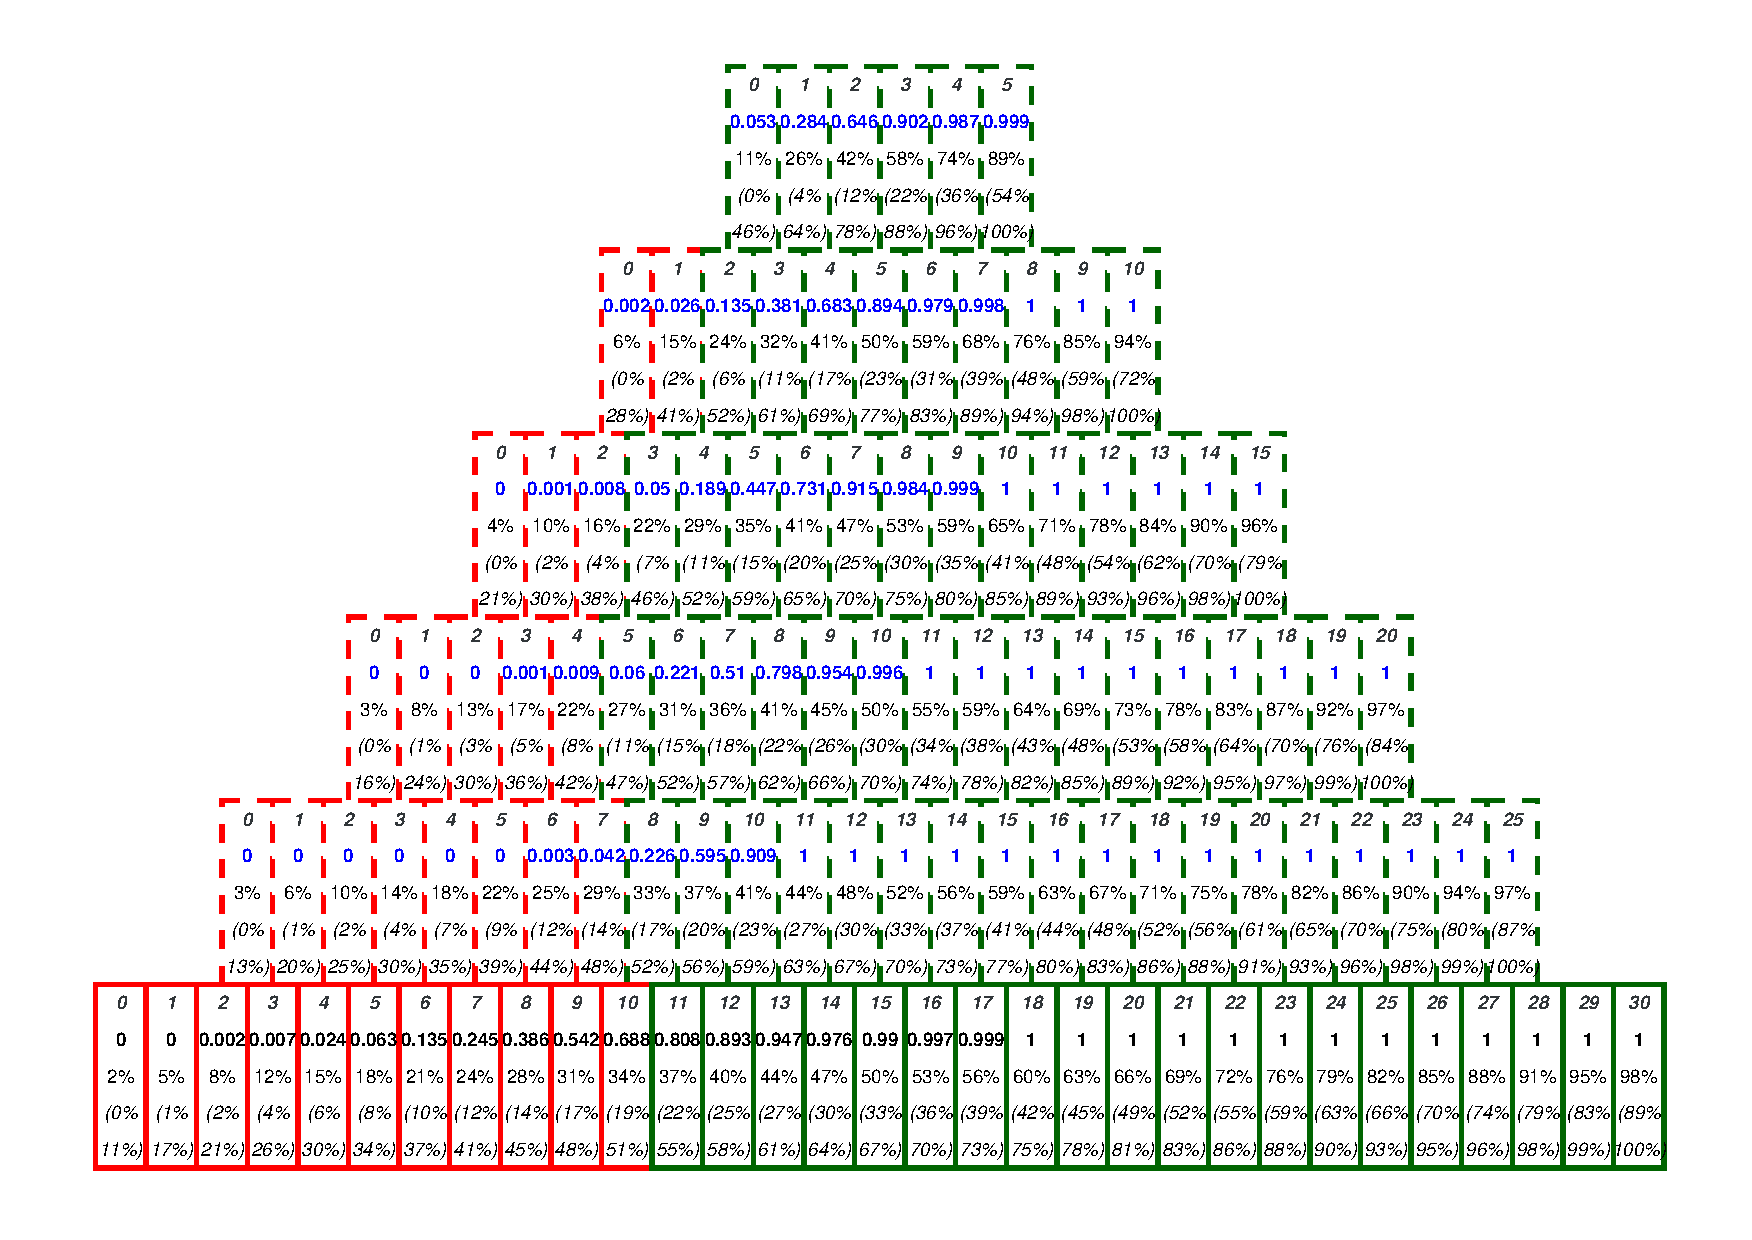
\includegraphics[width=25cm, height=15cm]{ETP-constructedNewFinalRule}
\end{sidewaysfigure}

\begin{sidewaysfigure}
	\centering
	\caption{Example of a constructed ETP with new target response rate.}
	\label{fig_etp:ConstructedETPNewTarget}
	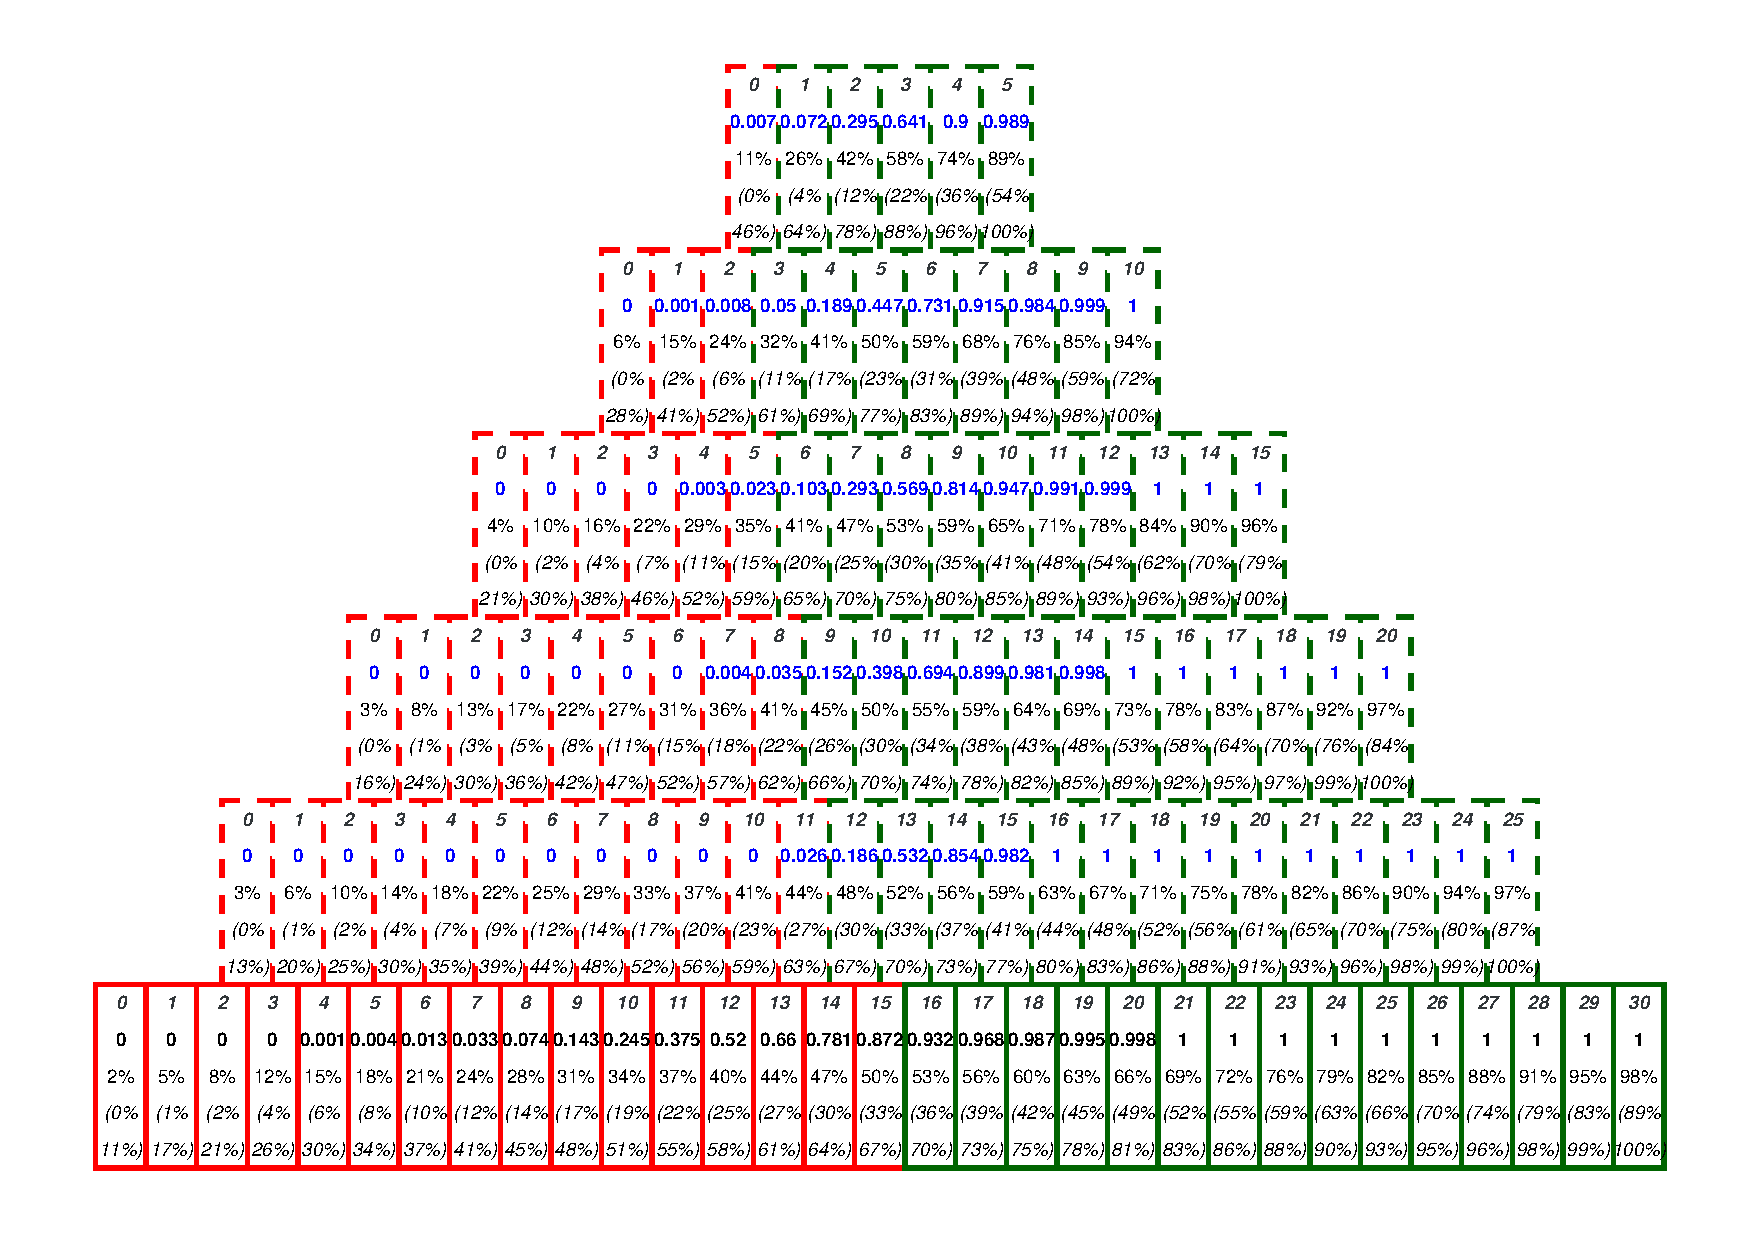
\includegraphics[width=25cm, height=15cm]{ETP-constructedNewFinalTarget}
\end{sidewaysfigure}  

\newpage

Here we have shown how ETPs are constructed and how they change and react to modifications in our decision rules. There are several other factors which can impact an ETP such as the prior used in the Beta-Binomial conjugate analysis as well as the timing of each interim analysis and the overall sample size of the trial. Changes to the prior will have an impact on all of the calculations as it is used to generate the posterior distribution on which all of the other calculations are based upon. Adding more interim analyses would add more rows to the plot and changing the sample size of the trial alters the number of cells in each row. 

Overall ETPs can be a useful tool during the design stages of a trial as we can experiment with different decision rules and see what practical affect it has on the trial in terms of the number of responses that need to be observed for a GO decision. They can be used to facilitate discussions with non statistical experts involved in the design of the trial. Much like dose transition pathways in a dose-finding trial they can also provide some transparency as to what decisions will be made and when they would be made. 

A single ETP also provides us with the ability to see how multiple different decision rules may change the outcome for a trial. If just the acceptable probability levels for the PPoS and final analysis, $t$ and $q$, are changing in the decision rule the impact of those changes should be apparent just by comparing the PPoS and posterior probability without the need of generating a whole new plot like we have in our example.

Whilst the calculations needed to produce these plots can be quite simple actually constructing the plots is not so trivial. In the next section we present an application we developed to overcome this issue and make ETPs easily accessible and producible. 


%----------------------------------------------------------------------------------------
%	SECTION 4
%----------------------------------------------------------------------------------------

\section{Development of a Web Application for ETPs}

Maybe scrap section specifically on determine and extend introduction for the development of a web application. 

Talk about how Cindy came up with this idea based on an extension to DTPs and had began implementing them in the design of some of her trials. Talk about Determine, MonoGerm, GLO-BNHL collegues were "hand generating" these ETPs. Demonstrated their usefulness when designing a trial and so that can be quite a tedious process. Calculations are easy with code but generating plot in power point etc. is effort. Perhaps show examples of what they had done (if allowed). Created a need to automate this process, needed to be accessible for multiple programming language users so converted into an app. Then extended that to also educate on these types of trial designs. 